\documentclass[10pt,a4paper,final]{article}
% cestina a fonty
\usepackage[utf8]{inputenc}
\usepackage[T1]{fontenc}
\usepackage{lmodern}
\usepackage{textcomp}
\usepackage{times}
\usepackage[czech]{babel}
% odsazeni prvniho radku
\usepackage{indentfirst}
% balicky pro odkazy
\usepackage[bookmarksopen,colorlinks,plainpages=false,urlcolor=blue,
unicode,linkcolor=black]{hyperref}
\pagestyle{plain}
\usepackage{url}
\DeclareUrlCommand\url{\def\UrlLeft{<}\def\UrlRight{>}
 \urlstyle{tt}}
% obrazky

\usepackage[dvipdf]{graphicx}
\usepackage{float}
% velikost stranky
\usepackage[top=2.5cm, left=2cm, text={17cm, 25cm}, ignorefoot]{geometry}

\begin{document}

%%%%%%%%%%%%%%%%%%%%%%%%%%%%%%%%%%%%%%%%%%%%%%%%%%%%%%%%%%%%%%%%%%%%%%%%%%%%%%%%
\thispagestyle{empty}

% titulni strana
\begin{center}
	\Huge \textsc{Vysoké učení technické v~Brně}\\
	\huge \textsc{Fakulta informačních technologií}\\
	\vspace{\stretch{0.382}}
	
\includegraphics[keepaspectratio]{images/fit.eps}\\
	\vspace{\stretch{0.382}}
	\Huge Analyzátor sieťovej prevádzky\\[5mm]
	\Large Projekt do predmetu Sieťové aplikácie a správa sietí (ISA)\\
	\vspace{\stretch{0.618}}
\end{center}
{\large \today \hfill Peter Tisovčík}
\newpage

% nastaveni cislovani
\pagestyle{plain}
\pagenumbering{arabic}
\setcounter{page}{1}

\tableofcontents
\newpage

%%%%%%%%%%%%%%%%%%%%%%%%%%%%%%%%%%%%%%%%%%%%%%%%%%%%%%%%%%%%%%%%%%%%%%%%%%%%%%%%
\section{Úvod} \label{sec:uvod}
%%%%%%%%%%%%%%%%%%%%%%%%%%%%%%%%%%%%%%%%%%%%%%%%%%%%%%%%%%%%%%%%%%%%%%%%%%%%%%%%

\noindent Cieľom projektu je vytvoriť konzolovú aplikáciu pre analýzu sieťovej prevádzky, ktorá je uložená vo formáte pcap. Aplikácia umožňuje analyzovať zachytené pakety a na základe zadaných filtrov a hodnôt vytvoriť štatistiku z týchto dát. Štatistiky sa zameriavajú na počet prenesených bajtov na jednotlivých vrstvách.
\\\\
Medzi podporované vrstvy patrí linková, sieťová a transportná vrstva. Na jednotlivých vrstvách sú podporované určité protokoly. Medzi podporované protokoly vo filtroch analyzátora na linkovej vrstve patrí MAC, na sieťovej vrstve IPv4, IPv6 a na transportnej vrtve TCP a UDP.
\\\\
Štatistku je možné vytvárať ako počet prenesených údajov k určitej adrese alebo ako zoznam desiatich adries, ktoré generujú najväčšie množstvo dát. Ak sa jedná o štatistiku pre určitú adresu výstupom je jeden riadok, ktorý obsahuje dve hodnoty oddelené medzerou. Prvá hodnota udáva súčet prenesených údajov od linkovej vrstvy. Druhá hodnota udáva množstvo dát v zadanom protokole. V prípade druhej štatistiky, ktorá zobrazuje zoznam desiatich adries, ktoré generujú najväčšie množstvo dát je tam pridaná adresa, ktorá generuje tieto dáta. Táto štatistika je uporiadaná podľa počtu prenesených údajov na linkovej vrstve zostupne. V prípade rozšírenia je možné spúšťať program s viacerými filtrami a hodnotami filtrov.

%%%%%%%%%%%%%%%%%%%%%%%%%%%%%%%%%%%%%%%%%%%%%%%%%%%%%%%%%%%%%%%%%%%%%%%%%%%%%%%%
\section{Spustenie aplikácie}
%%%%%%%%%%%%%%%%%%%%%%%%%%%%%%%%%%%%%%%%%%%%%%%%%%%%%%%%%%%%%%%%%%%%%%%%%%%%%%%%

\noindent Aplikáciu je možné spustiť len z konzoly, neobsahuje grafické užívateľské rozhranie. Pred spustením je potrebné aplikáciu preložiť pomocou priloženého \texttt{Makefile} súboru príkazom \texttt{make}. Potrebné súbory je možné zabaliť do archívu \texttt{make tar}. Na odstránenia vygenerovaných súborov je možné použiť \texttt{make clean}, ktorý odstráni všetky súbory, ktoré sa dajú vygenerovať.
\\\\
\texttt{./analyzer [-i <pcap súbor>] [-f <typ filtra>] [-v <hodnota filtra>] [-s] [-d]}
\\\\
Popis prepínačov:
\begin{itemize}
	\item \texttt{-i <súbor>} pcap súbor obsahujúci dáta k analýze
	\item \texttt{-f <mac|ipv4|ipv6|tcp|udp>} položky v sieťovom rámci podľa, ktorej sa bude vyhľadávať, položky je možné oddeliť bodkočiarkou \texttt{mac;ipv4;tcp}
	\item \texttt{-v <hodnota filtra>} udáva hodnotu zadaného filtra, viacej hodnôt je oddelených čiarkou a jednotlivé typy hodnôt sú oddelené bodkočiarkou \texttt{ff:ff:ff:ff:ff:ff, e0:05:12:45:65:45;192.168.0.11;3300}
	\item \texttt{-v top10}  zobrazenie štatistitik  pre adresy s najväčším množstvom dát
	\item \texttt{-s} filtér, ktorý bude počítať štatistiky len zo zdrojových adries
	\item \texttt{-d} filtér, ktorý bude počítať štatistiky len z cieľových adries
\end{itemize}

Hodnotu filtra \texttt{-v top10} nie je možné kombinovať s viacerými typmi fitra, je podporovaný len jeden typ filtra. Filtér pre zdrojové a cieľové adresy je možné kombinovať.
\\\\
Hodnoty filtra \texttt{-v <hodnota filtra>} sa zapisujú bez medzier a majú nasledujúce pravidlá:
\begin{itemize}
	\item \texttt{MAC} 48-bitové číslo, ako oddeľovať dvojíc je použitá dvojbodka \texttt{e0:05:12:45:65:45}
	\item \texttt{IPv4} 32-bitové číslo zapísané po jednotlivých bajtoch, oddelené bodkou \texttt{192.168.5.111}
	\item \texttt{IPv6} 128-bitové číslo zapísané ako osem skupín po štyroch hexadecimálnych čísliciach, oddeľovať je dvojbodka, je možné použiť skrátený zápis  \texttt{0000:0000:0000:0000:0000:0000:0000:0001,::1}

\end{itemize}

\newpage
%%%%%%%%%%%%%%%%%%%%%%%%%%%%%%%%%%%%%%%%%%%%%%%%%%%%%%%%%%%%%%%%%%%%%%%%%%%%%%%%
\section{Popis problematiky}
%%%%%%%%%%%%%%%%%%%%%%%%%%%%%%%%%%%%%%%%%%%%%%%%%%%%%%%%%%%%%%%%%%%%%%%%%%%%%%%%
\subsection{Libpcap formát}

Pcap je formát súboru, ktorý je používaný pre odchytávanie sieťovej komunikácie. Nejedná sa o štandard pre odchytenú komunikáciu\cite{pcapformat}.
\\\\
Pcap súbor má presne definovanú štruktúru. Každý pcap súbor sa skladá z globálnej hlavičky a odchytených dát. Globálna hlavička uchováva informácie o celom súbore. Z hravičky je možné zistiť, typ súboru, maximálnu veľkosť odchytených dát, verziu ale aj typ odchytenej komunikácie na linkovej vrstve. Za globálnou hlavičkou sa nachádzajú dáta každý zachytený údaj obsahuje hlavičku, ktorá ho reprezentuje a potom samostatné dáta. Z hlavičky je možné vyčítať veľkosť dát  ale aj čas zachytenia daného paketu. 

\begin{figure}[H]
	\centering
	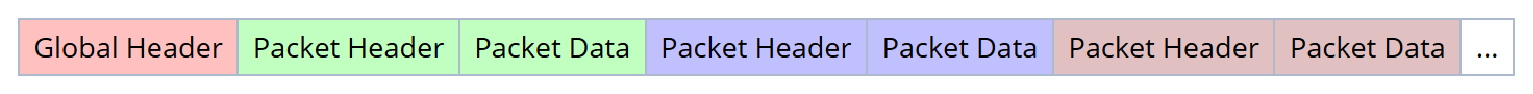
\includegraphics[scale=0.665, keepaspectratio]{images/pcap.eps}
	\caption{Formát pcap súboru\cite{pcapformat}}
\end{figure}

\subsection{Linková vrstva}
\subsubsection{Ethernet II - Ethernetový rámec}

Ethernet patrí medzi základné protokoly na linkovej vrstve pre posielanie dát. Ethernetový rámec obsahuje zdrojovú a cieľovú MAC adresu, pred ktorými sa ešte nachádza preambula a oddeľovač začiatku rámca (SFD). Jednotlivé adresy umožňujú adresovať zariadenia na linkovej vrstve a majú veľkosť 48-bitov. Za adresami sa nachádza typ , ktorý identifikuje ethernetový rámec. Obsahuje protokol, ktorý sa nachádza na nasledujúcej vrstve. Na základe tohto typu je možné zistiť, či sa jedná o rámec s VLAN označením. Za týmto typom sa nachádzajú dáta vyššej vrstvy, ktoré boli odchytené. Za dátami sa nachádza kontrolná súčet rámca pre určenie, či nedošlo k poškodeniu pri prenose\cite{ethernetframe}.
\begin{figure}[H]
	\centering
	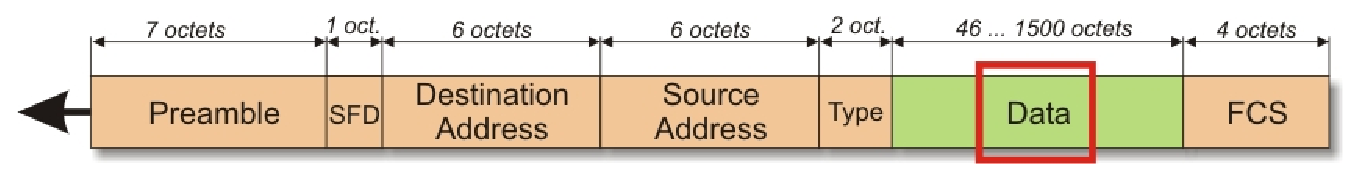
\includegraphics[scale=0.665, keepaspectratio]{images/ethernet.eps}
	\caption{Formát Ethernet II rámca\cite{ethernetframeimg}}
\end{figure}

\subsubsection{IEEE 802.1Q - VLAN Tagging}

Štandard, ktorý umožňuje jednu fyzickú ethernetovú sieť rozdeliť na viacej logických sietí VLAN pomocou rozšírenej hlavičky\cite{osemdvavlan}. IEEE 802.1Q vkladá do hlavičky informáciu o identifikácií VLAN. Je možné posielať v sebe zabalených viacej VLAN hlavičiek, aby bolo možné jednolivé pakety, ktoré obsahujú VLAN preposlať ďalšou VLAN ďalej do siete.
\begin{figure}[H]
	\centering
	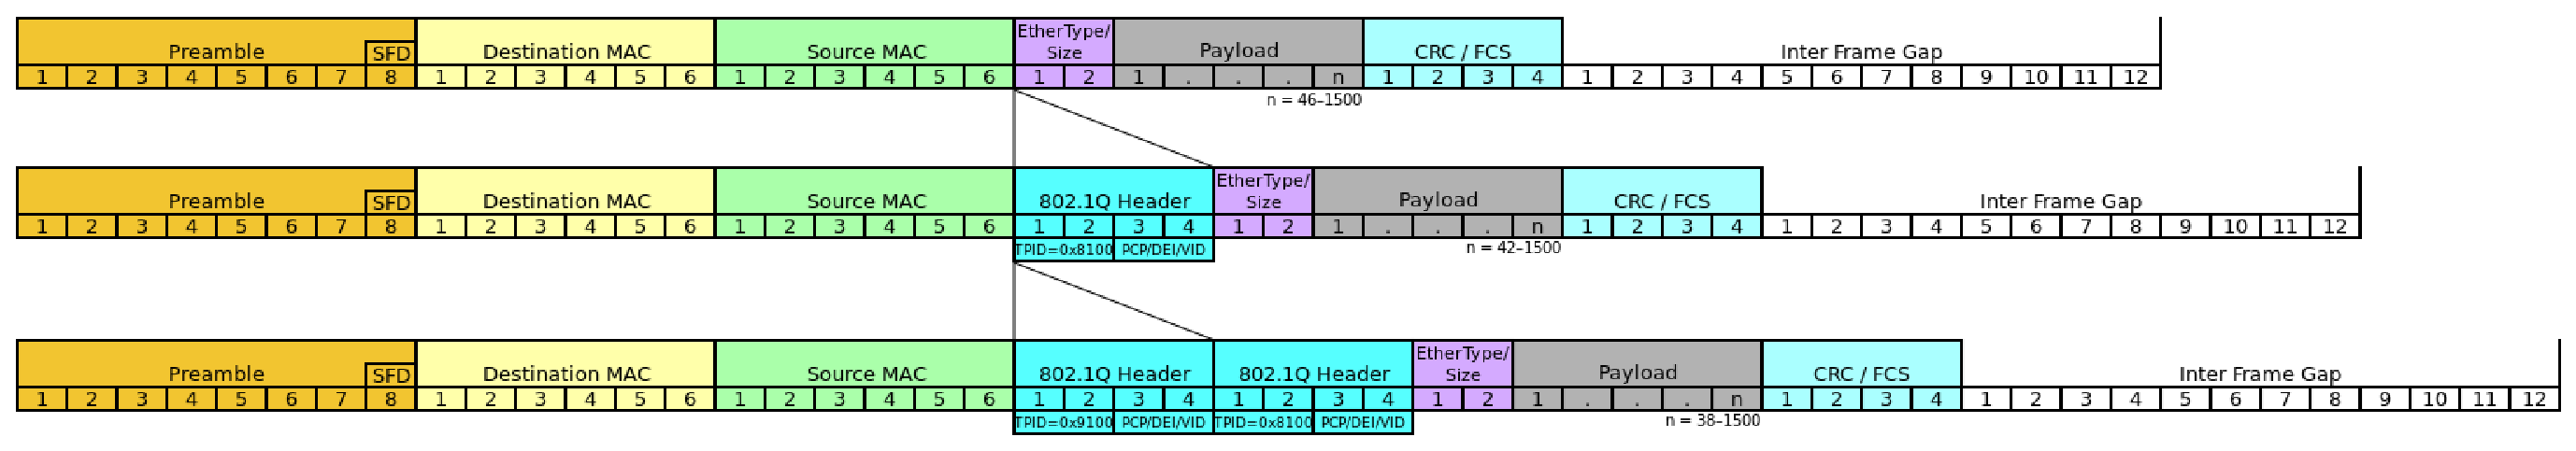
\includegraphics[scale=0.37, keepaspectratio]{images/vlan.eps}
	\caption{IEEE 802.1Q  VLAN Tagging \cite{osemdvavlan}}
\end{figure}

\newpage
\subsection{Sieťová vrstva}
\subsubsection{IPv4 protokol}
IPv4 protokol slúži na adresovanie zariadení na sieťovej vrstve. Dneska sa nahrádza IPv6, ktorá ma väčší adresovací priestor. IPv4 používa 32-bitové adresy. Táto adresa tvori unikátny identifikátor na základe, ktorého je možné identifikovať zariadenie a poslať mu údaje.
\\\\
Hlavička je dlhá 20 bajtov(oktetov). Na začiatku sa nachádza verzia protokolu, ďalej sa tu nachádzajú príznaky pre riadenie fragmentácie, identifikátor paketu, protokol na ďalšej vrstve a zdrojová a cieľová adresa. Za zdrojovou a cieľovou adresou sa nachádzajú dáta a v prípade, že dáta nie sú zarovnané na  32-bitov sú doplnené paddingom.\cite{ipv4-img}
\begin{figure}[H]
	\centering
	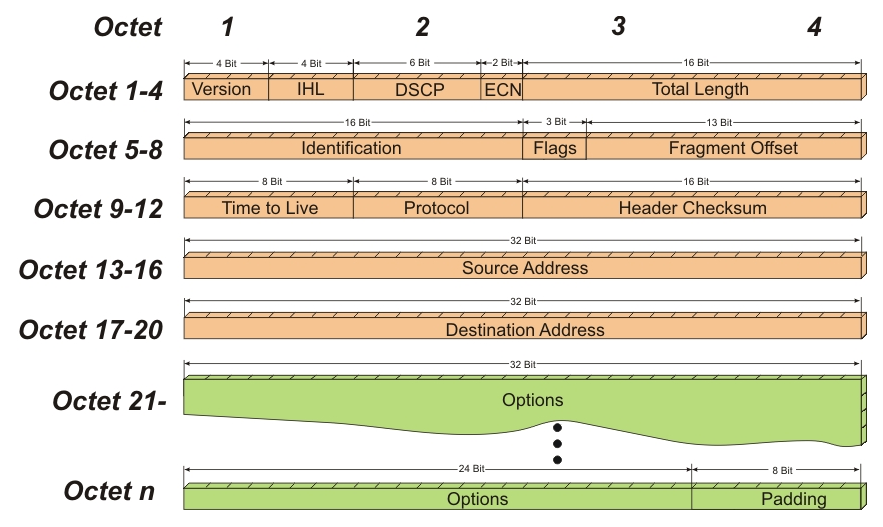
\includegraphics[scale=0.8, keepaspectratio]{images/ipv4.eps}
	\caption{IPv4 hlavička\cite{ipv4-img}}
\end{figure}

\subsubsection{IPv6 protokol}
IPv6 protokol slúži na adresovanie zariadení na sieťovej vrstve. Nahradzuje staršiu verziu IPv4. Podobne ako IPv4 obsahuje verziu protokolu, príznaky, dĺžku dát, adresy a nasledujúcu hlavičku. Od predchádzajúcej verzie sa nelíši len vo veľkosti adries, ktoré su 128-bitové ale aj v možnosti reťaziť jednotlivé hlavičky za seba.
\begin{figure}[H]
	\centering
	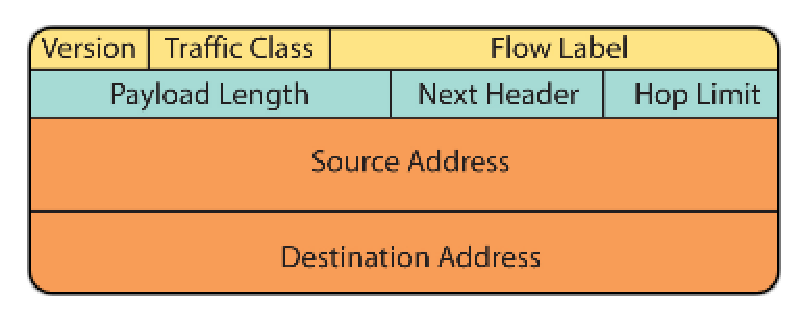
\includegraphics[scale=0.60, keepaspectratio]{images/ipv6.eps}
	\caption{IPv6 hlavička\cite{ipv6-img}}
\end{figure}


\subsubsection{ARP a RARP protokol}
Protokol ARP slúži na získanie linkovej adresy sieťového zariadenia. Umožňuje na základe cieľovej IP adresy zistiť MAC adresu, aby sme mohli IP paket zabaliť do ethernetového rámca. V prípade, že je známa MAC adresa a chceme zistiť aká IP adresa k danej MAC adrese je priradená je možné na tento účel použiť RARP protokol\cite{arp}.

\subsection{Transportná vrstva}
\subsubsection{TCP protokol}
TCP protokol vytvára spojenia a garantuje spoľahlivé doručovanie paketov a zároveň garantuje, že packety budú doručené v správnom poradí. Je to veľmi dôležité pre niektoré aplikácie, kde je potrebné mať dáta doručené správne. Medzi také aplikácie patrí napríklad prehliadač webu alebo email. Hlavička obsahuje zdrojový, cieľový port a informácie potrebné pre vytvorenie spojenia a kontrolu správnosti daných paketov. TCP hlavička neobsahuje veľkosť dát, len veľkosť hlavičky. Na konci hlavičky sa nachádza kontrolný súčet, ktorý zaisťuje kontrolu správnosti hlavičky. Za hlavičkou nasledujú dáta.

\begin{figure}[H]
	\centering
	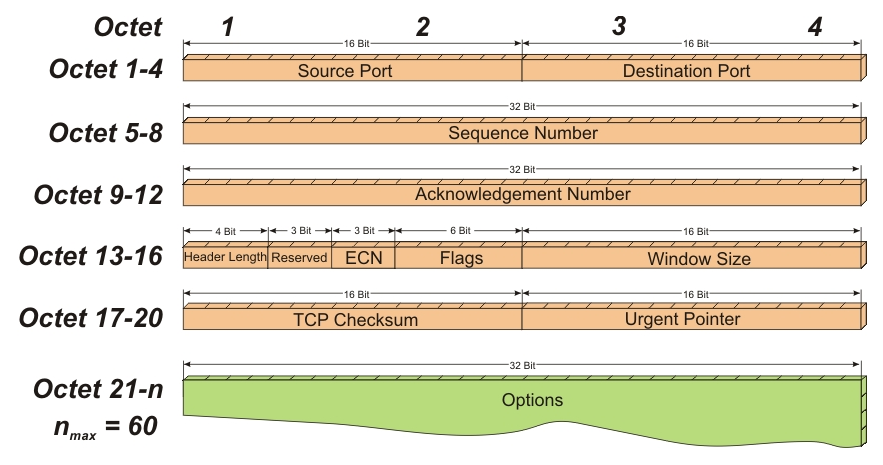
\includegraphics[scale=0.63, keepaspectratio]{images/tcp.eps}
	\caption{TCP hlavička\cite{ipv6-img}}
\end{figure}

\subsubsection{UDP protokol}
UDP protokol narozdiel od TCP protokolu nezaručuje, že odoslané dáta búdu doručené. Na prvý pohľad sa zdá, že taký protokol nemá využitie ale narozdiel od TCP nemá takú veľkú réžiu pri prenášaní. Z toho vyplýva, že aj keď je nespoľahlivý je ho možné využiť pri veľkých tokoch dát. Používa sa hlavne tam, kde nevadí, že sa niektoré dáta nedoručia ako napríklad pozeranie videa alebo VoIP. Hlavička obsahuje len zdrojovú a cieľovú adresu, dĺžku dát a kontrolný súčet hlavičky. Za hlavičkou nasledujú dáta.
\begin{figure}[H]
	\centering
	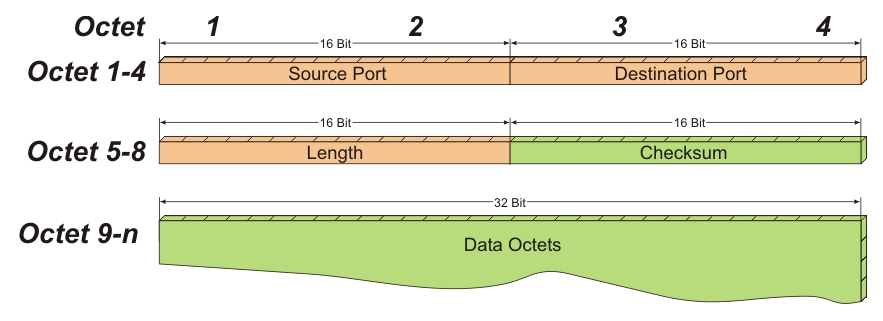
\includegraphics[scale=0.63, keepaspectratio]{images/udp.eps}
	\caption{UDP hlavička\cite{udpprotocol}}
\end{figure}


%%%%%%%%%%%%%%%%%%%%%%%%%%%%%%%%%%%%%%%%%%%%%%%%%%%%%%%%%%%%%%%%%%%%%%%%%%%%%%%%
\section{Popis implementácie}
%%%%%%%%%%%%%%%%%%%%%%%%%%%%%%%%%%%%%%%%%%%%%%%%%%%%%%%%%%%%%%%%%%%%%%%%%%%%%%%%

\noindent Sieťový analyzátor je napísaný v programovacom jazyku C++ a skladá sa z niekoľkých logických častí. Na parsovanie argumentov je využitá vstavaná funkcia, ktorá je upravená aby vyhovovala zadaniu. V rámci parsovania argumentov sa kontroluje správnosť zadaných parametrov a filtrov. Kontroluje sa, či boli zadané správne hodnoty v správnom poradí a či sa niektoré argumenty neopakujú. Pri uchovávaní hodnôt filtrov sa údaje ukladajú v jednotnom formáte, ktorý zaručí, že pri porovnávaní hodnoty filtra a hodnoty z paketu nemôže dôsť k problémom. Ďalšou dôležitou časťou je parsovanie jednotlivých paketov zo súboru. Pre parsovanie údajov z paketov bol použitý návrhový vzor \texttt{factory}, ktorý mi umožňuje volať metódu bez bez nutnosti vedieť, o ktorý objekt sa jedná. V tomto prípade sa jedná o jednotlivé sieťové vrstvy, ktoré sa v sebe implementujú parsovanie jednotlivých protokolov na danej vrstve. Jednotlivé vrstvy vracajú rovnaký objekt, ktorý v sebe uchováva informácie o danej vrstve ale aj o vrstve, ktorá sa nachádzala pred ňou. Pre vytvorenie tohto objektu je potrebné len predať dáta paketu a jeho hlavičku. Tymto spôsobom je oddelená časť na spracovanie údajov a vytvárania štatistiky. Štatistiku tvori veľmi jednoduchá množina hodnôt, ktorá sa dá vypísať. Porovnávanie zadanej adresy ako hodnotu filtra a vyparsovanej adresy sa vykonáva v \texttt{main()}.

\subsection{Spracovanie argumentov}
Pred spracovaním argumentov je potrebné triede \texttt{ArgumentParser} nastaviť argumenty, ktoré môže parsovať a ich jednotlivé vlastnosti. Následne je možné zahájiť spracovanie argumentov. 
Na spracovanie argumentov slúži trieda \texttt{ArgumentParser}, ktorá obsahuje metódu \texttt{validateArguments()}, po jej zavolaní sa zaháji proces kontroly argumentov. Najprv je potrebné načítať a rozparsovať údaje z reťazca \texttt{extractArguments()}. Po uložení jednotlivých údajov o argumentoch sa skontrolujú zadané filtre, či sú podporované a či sú správne zapísané metódou \texttt{checkFilterExists()}. Ďalej je potrebné zistiť, či sa má filter aplikovať na zdrojové alebo cieľové adresy, prípadne na obe. Po týchto kontrolách nasleduje kontrola o aký typ štatistiky sa jedná, ak sa jedná o \texttt{top10} metóda \texttt{checkIsTop10()} nastaví premennú, ktorá indikuje, že sa má vypísať táto štatistika. Nakoniec sa skontrolujú hodnoty filtrov metódou \texttt{checkFilterValues()}. Pri kontrole hodnôt zadaných filtrov sa kontroluje, či daný filtér zodpovedá zadaným hodnotám a validnosť jednotlivých hodnôt. Ak je hodnota validná uloží sa jej adresa k požadovanému protokolu.


\subsection{Spracovanie paketov}
Pre spracovanie jednotlivých vrstiev je pripravené rozhranie \texttt{LayerMessageFactory}, ktoré je treba naimplementovať pre jednotlivé vrstvy. Toto rozhranie obsahuje metódu \texttt{create()}, ktorá spracuváva jednotlivé dáta a zároveň vracia rozparsované dáta v objekte. Pred zahájením parsovania paketov je nutné jednotlivé vrstvy zaregistrovať \texttt{register()} do \texttt{GenericLayerMessageFactory}, ktorá sa stará o správu jednotlivých vrstiev. Trieda obsahuje mapu, kde sa nachádzajú jednotlivé vrstvy a v tele \texttt{create()} je možné volať jednotlivé vrstvy. Z tejto metódy je možné volať implementácie jednotlivých vrstiev. Pri spracovaní jednotlivých vrstiev sa postupuje sekvenčne a najprv sa spracuje linková, sieťová a nakoniec transportná vrstva. Linková vrstva načíta celý obsah paketu do \texttt{LayerMessage}, ktorá uchováva adresy na danej vrstve, ich dĺžky a dáta poslednej spracovanej vrstvy. Pri spracovaní jednotlivých vrstiev sa tento objekt predáva a dopĺňa sa o adresy a dĺžky, ktoré sa načítajú z paketu. Pri ukladaní adries sa používajú statické metódy z triedy \texttt{ArgumentValidator} pre zjednotenie formátu adries kôli jednoduchšiemu porovnávaniu. 

\subsection{Naplnenie štatistiky}
Štatistika sa plní v \texttt{main()}, kde sa v cykle vracajú objekty \texttt{LayerMessage}, ktoré obsahujú adresy zo zadaným protokolom a jednotlivé dĺžky dát. Následne sa prejde všetkými filtrami, ktoré boli zadané. Pri prechode sa hľadá zhoda adries na danej vrstve a zadaných adries ktoré boli zadané ako parametre programu. V prípade, že sa jedná o rozšírenie, tak sa pri jednotlivých prechodoch kontrolujú jednotlivé vrstvy od linkovej až po transportnú. Ak sa na niektorej vrstve nenachádza daná adresa je paket preskočený. Metóda \texttt{extractHighestLayer} zistí zo zadaných filtrov najvyššiu vrstvu, po ktorú má kontrolovať a ak narazí na ňu zapíšu sa údaje do štatistiky. Štatistika je tvorená jednoduchou množinou hodnôt, do ktorej je možné vkladať údaje metódou \texttt{insert()}. Pri vkladaní sa použije adresa ako kľúč aby bolo možné pri ďalšom vkladaní upraviť hodnotuuž existujúcej adresy. Trieda pre štatistiku \texttt{Statistics} obsahuje metódu na zotriedenie štatistiky, výpis top10 alebo na výpis obyčajnej štatistiky.

%%%%%%%%%%%%%%%%%%%%%%%%%%%%%%%%%%%%%%%%%%%%%%%%%%%%%%%%%%%%%%%%%%%%%%%%%%%%%%%%
\section{Testovanie}
%%%%%%%%%%%%%%%%%%%%%%%%%%%%%%%%%%%%%%%%%%%%%%%%%%%%%%%%%%%%%%%%%%%%%%%%%%%%%%%%
Pre otestovanie programu boli vytvorené testy, ktoré boli rozdelené na dve časti. Prvá časť tvorila testovanie argumentov, ich správnosť alebo nesprávnosť. Tieto testy sa zameriavali na kontrolu, či existujú parametre, hodnoty, či boli zadané správne alebo či nebol zabudnutý nejaký prepínač. Druhá časť testov tvorí testovanie jednotlivých pcap súborov a jednotlivých výstupov. Výstupy sa porovnávali s referenčnými výstupmi, ktoré boli vytvorené zisťovaním pomocou wireshaku alebo priamo programom pre analýzu. Všetky testy prebiehali automaticky a boli napísané ako bash script.
\\\\
Ukážka testov:
\\\\
\texttt{testcompare "\$\{BIN\} -i traffic.pcap -f mac -v 1c:1b:0d:04:7d:50 -s -d
      " \$OK " file31" }
\texttt{test "\$\{BIN\} -i file.pcap -f mac -v -s" \$\{ERR\} "Chýba hodnota filtra."}




%%%%%%%%%%%%%%%%%%%%%%%%%%%%%%%%%%%%%%%%%%%%%%%%%%%%%%%%%%%%%%%%%%%%%%%%%%%%%%%%
\section{Záver}
%%%%%%%%%%%%%%%%%%%%%%%%%%%%%%%%%%%%%%%%%%%%%%%%%%%%%%%%%%%%%%%%%%%%%%%%%%%%%%%%
Program funguje ako jednoduchý analyzátor pcap súborov, nad ktorým je možné robiť štatistiky na základe zadaných filtrov a ich hodnôt. Je navrhnutý ako objektový orientovaný a jeho ďalšie rozširovanie nie je problém. Implementuje rozšírenie a tým pádom je možné vypisovať štatistiky na základe viacerých filtrov a hodnôt. Pre otestovanie funkcionality boli vytvorené vlastné testy a odchytené vlastné pcap súbory.


\newpage
\bibliographystyle{czplain}
\renewcommand{\refname}{Literatura}
\raggedright
\bibliography{literatura}
\end{document}
